% !TeX document-id = {b9013c51-794e-4cf8-8a3e-aca2d69fba10}
% !TeX TXS-program:compile = txs:///pdflatex/[--shell-escape]

\documentclass{article}

\usepackage[utf8]{inputenc}
\usepackage[T1]{fontenc}
\usepackage{lmodern}
\usepackage[french]{babel}
\usepackage{multicol}
\usepackage{amsmath}
\usepackage{amssymb}
\usepackage{enumitem}
\numberwithin{equation}{section}
\usepackage{algorithm}
\usepackage{algorithmic}
\usepackage{graphicx}
\usepackage{float}
\usepackage{moreverb}
\usepackage{url}
\usepackage{subcaption}
\setlength\parindent{0pt}
\usepackage{bbm}
\usepackage{booktabs}
\usepackage{longtable}
\usepackage{array}
\usepackage{multirow}
\usepackage[table]{xcolor}
\usepackage{wrapfig}
\usepackage{colortbl}
\usepackage{pdflscape}
\usepackage{tabu}
\usepackage{threeparttable}
\usepackage{threeparttablex}
\usepackage[normalem]{ulem}
\usepackage{makecell}
\usepackage{breakcites}
\usepackage[htt]{hyphenat}
\usepackage{fancyvrb}
\usepackage{algorithm}
\usepackage{algorithmic}
\usepackage{listingsutf8}
\usepackage{listings}
\usepackage{color}
\usepackage{nameref}
\usepackage{minted}


\setlength{\parskip}{1em}
\usepackage[margin=1in]{geometry}

\definecolor{dkgreen}{rgb}{0,0.6,0}
\definecolor{gray}{rgb}{0.5,0.5,0.5}
\definecolor{mauve}{rgb}{0.58,0,0.82}

\usepackage{hyperref}
\hypersetup{
	colorlinks=true,
	linkcolor=blue,
	filecolor=magenta,      
	urlcolor=cyan,
}

\urlstyle{same}

\begin{document}
\begin{titlepage}
	\centering % Centre everything on the title page
	
	\scshape % Use small caps for all text on the title page
	
	\vspace*{\baselineskip} % White space at the top of the page
	
	%------------------------------------------------
	%	Title
	%------------------------------------------------
	
	\rule{\textwidth}{1.6pt}\vspace*{-\baselineskip}\vspace*{2pt} % Thick horizontal rule
	\rule{\textwidth}{0.4pt} % Thin horizontal rule
	
	\vspace{0.75\baselineskip} % Whitespace above the title
	
	{\LARGE TRAVAIL	PRATIQUE \#3 - CLASSIFICATION DE TEXTES ET ANALYSE DE SENTIMENTS DANS LES CONVERSATIONS\\} % Title
	\vspace{0.5\baselineskip} % Whitespace before the editors
	\raisebox{-1pt}{
\includegraphics[height=20pt, width=20pt]{GitHub-Mark-32px}}\ 
	\href{https://github.com/Samuel-Levesque/ift-7022_devoir_3}{Lien GitHub}
	\vspace{0.75\baselineskip} % Whitespace below the title
	
	\rule{\textwidth}{0.4pt}\vspace*{-\baselineskip}\vspace{3.2pt} % Thin horizontal rule
	\rule{\textwidth}{1.6pt} % Thick horizontal rule
	
	\vspace{2\baselineskip} % Whitespace after the title block
	
	%------------------------------------------------
	%	Subtitle
	%------------------------------------------------
	{\scshape\Large William Bourget\\111 129 490\\Samuel Lévesque\\111 127 772\\} % Editor list
	\vspace{0.5\baselineskip} % Whitespace before the editors
	Pour le cours IFT-7022\\
	Techniques et applications du traitement de la langue naturelle \\% Subtitle or further description
	
	\vspace*{3\baselineskip} % Whitespace under the subtitle
	
	%------------------------------------------------
	%	Editor(s)
	%------------------------------------------------
	
	Présenté le 14 décembre 2018 au professeur
	
	\vspace{0.5\baselineskip} % Whitespace before the editors
	
	{\scshape\Large Luc Lamontagne \\} % Editor list
	
	\vspace{0.5\baselineskip} % Whitespace below the editor list
	
	\textit{Département d'informatique et de génie logiciel\\Faculté des sciences et de génie\\Université Laval} % Editor affiliation
	
	\vfill % Whitespace between editor names and publisher logo
	
	%------------------------------------------------
	%	Publisher
	%------------------------------------------------
	
        
        
\includegraphics[height=1cm, width=2.5cm]{UL_P.pdf}\\
        Faculté des sciences et de génie\\
        Université Laval\\
        Automne 2018       
\end{titlepage}

\newpage
\tableofcontents
\newpage

\section{Introduction}
Ce projet porte sur la seconde suggestion de travaux proposée sur le site de cours: \emph{ Classification de texte et analyse de sentiments dans les conversations}. Le but consiste à prédire le sentiment (happy, angry, sad) dégagé dans un échange de 3 textos. Un corpus d'entraînement est fourni pour réaliser la tâche. 

Le code est constitué de plusieurs fichiers. Le plus important est celui nommé \emph{Main}. C'est le seul que l'on ait besoin de rouler. Différentes options d'exécution sont offertes:

%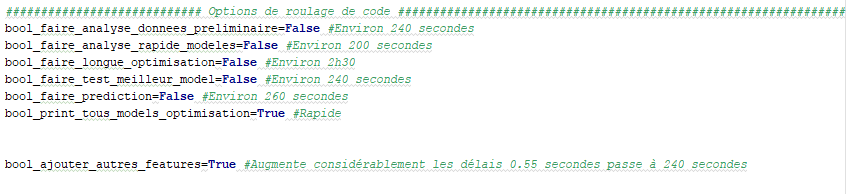
\includegraphics[width=\linewidth,height=6cm]{images/list_bool}

\begin{minted}[breaklines]{python}
############################ Options d'exécution du code ######################
bool_faire_analyse_donnees_preliminaire = True  # Environ 240 secondes
bool_faire_analyse_rapide_modeles = True  # Environ 200 secondes
bool_faire_longue_optimisation = True  # Environ 2h30
bool_faire_test_meilleur_model = True  # Environ 240 secondes
bool_faire_prediction = True  # Environ 260 secondes
bool_print_tous_models_optimisation = True  # Rapide
bool_ajouter_autres_features = True  # Augmente considérablement les délais .55 secondes passe à 240 secondes
\end{minted}

%\lstinputlisting[caption=Options d'exécution du code, style=customc]{exec.c}

\verb|bool_faire_analyse_donnees_preliminaire = True| permet de faire l'analyse préliminaire des données présentée dans la section \nameref{sec:analyse_prelim}. 

\verb|bool_faire_analyse_rapide_modeles = True| permet de faire l'analyse présentée dans la sous-section \nameref{subsec:modeles}. 

\verb|bool_faire_longue_optimisation = True| permet de compléter l'optimisation présentée dans la sous section \nameref{subsec:modeles}. 

\verb|bool_faire_test_meilleur_model = True| permet d'obtenir les résultats présentés dans la sous-section \nameref{subsec:simulation}. 

\verb|bool_faire_prediction = True| permet de faire les prédictions présentées dans la sous-section \nameref{subsec:predictions}. 

\verb|bool_print_tous_models_optimisation = True| permet d'afficher tous les résultats possibles de modèles créés dans la sous-section \nameref{subsec:optimisation}.

\verb|bool_ajouter_autres_features = True| permet de transformer les \emph{emojis} en texte et d'ajouter les attributs supplémentaires présentés à la section \nameref{sec:analyse_prelim}.

%\newpage

\section{Analyse préliminaire des données} \label{sec:analyse_prelim}
\subsection{Analyse des \emph{emojis} et des binettes} \label{subsec:emojis}
En regardant rapidement les données fournies dans le fichier \emph{train.txt}, on peut voir que les échanges de textos sont très courts. Également, il y a beaucoup d'\emph{emojis} et de binettes créés à partir de caractères spéciaux (ex: :), :D, :(, :-)).

On peut regarder le nombre de textes avec la présence d'au moins un emoji particulier selon chaque classe pour voir si ceux-ci semblent être beaucoup plus présents dans une classe ou une autre. Les résultats obtenus pour quelques emojis testés se trouvent dans la table \ref{table:emojis}

% Please add the following required packages to your document preamble:
% \usepackage{booktabs}
\begin{table}[]
	\centering
	\caption{Comptes préliminaires d'emojis}
	\label{table:emojis}
	\begin{tabular}{@{}lllll@{}}
		\toprule
		Emoji testé & Angry & Happy & Sad & Others \\ \midrule
		
\includegraphics[height=0.5cm]{images/heart}          & 8     & 31    & 13  & 41     \\
		
\includegraphics[height=0.3cm]{images/broken_heart}          & 2     & 0     & 64  & 3      \\
		
\includegraphics[height=0.3cm]{images/heart_eyes}          & 10    & 88    & 10  & 92     \\
		
\includegraphics[height=0.3cm]{images/sad}          & 15    & 1     & 282 & 15     \\
		
\includegraphics[height=0.3cm]{images/laughter}          & 59    & 989   & 49  & 197    \\
		
\includegraphics[height=0.3cm]{images/angry}          & 156   & 6     & 18  & 10     \\ \bottomrule
	\end{tabular}
\end{table}

%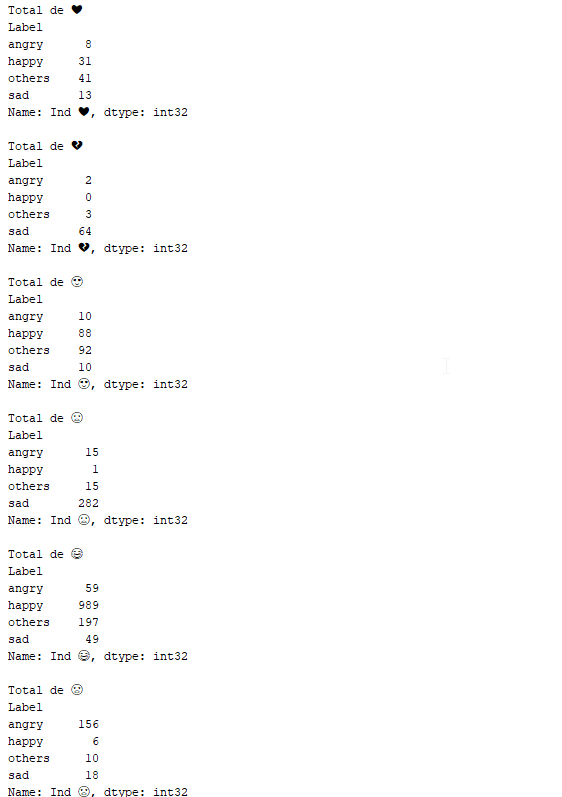
\includegraphics[width=\linewidth,height=15cm,keepaspectratio]{images/analyse_emojis}

À première vue, les emojis semblent avoir un impact important. Par exemple, le coeur brisé et le bonhomme triste sont souvent utilisés dans des échanges de textos tristes alors que celui qui fait un sourire est utilisé pour les échanges neutres ou joyeux. Il semble donc pertinent de convertir tous les emojis en texte pour les traiter avec un objet de compte de mots.

On peut également tenter de repérer les binettes créés à partir de caractères spéciaux. Pour parvenir à les identifier, on peut utiliser une expression régulière qui identifie les séries de 2 à 6 caractères spéciaux. On voit ici ladite expression régulière avec la liste des chaînes de caractères ainsi extraites.
\begin{verbatim}
reg ex : [^\w\s\d]{2,6}
\end{verbatim}

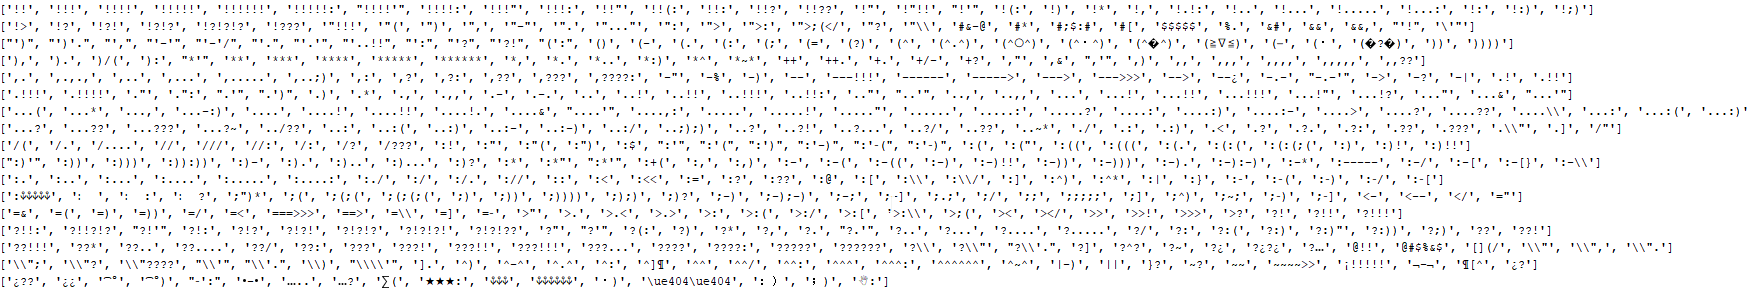
\includegraphics[width=\linewidth,height=7cm]{images/analyse_list_car_speciaux}

À partir de cela, on peut tenter d'identifier toutes les chaînes qui semblent intéressantes de façon manuelle. Pour voir rapidement si ces chaînes de caractères pourraient être discriminantes, on fait une analyse des comptes selon nos quatre classes. La table .... présente les résultats les plus intéressants.

\begin{figure}[h!] %h: place figure here if possible, t: top, b:bottom, !:over-ride default placement
	\begin{minipage}[b]{0.3\textwidth}
		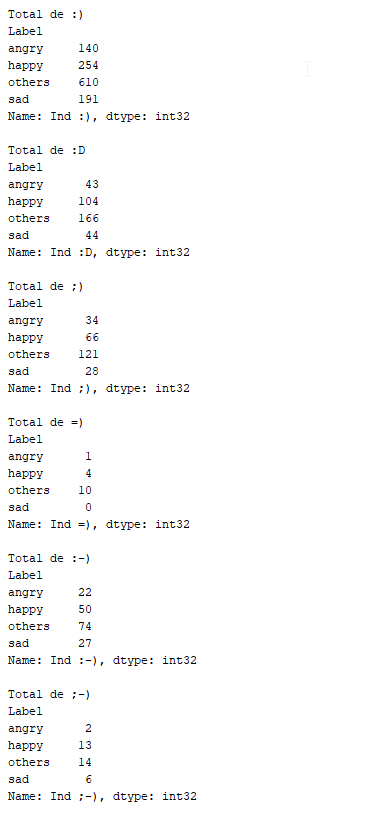
\includegraphics[width=\textwidth,height=14cm]{images/analyse_emojis_car_pos}
	\end{minipage}
	\hfill
	\begin{minipage}[b]{0.3\textwidth}
		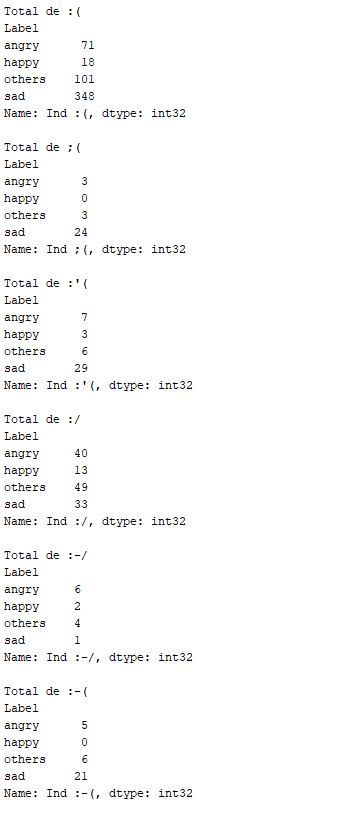
\includegraphics[width=\textwidth,height=14cm]{images/analyse_emojis_car_neg}
	\end{minipage}
	\hfill
	\begin{minipage}[b]{0.3\textwidth}
		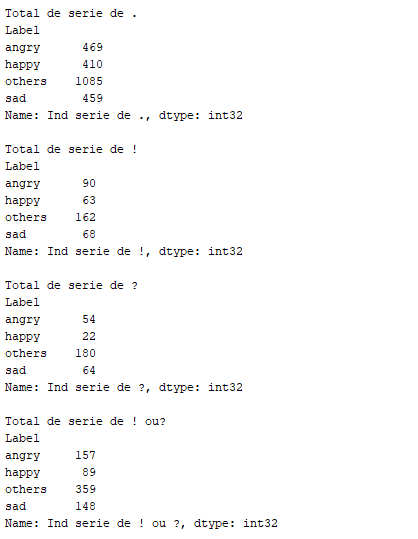
\includegraphics[width=\textwidth,height=14cm]{images/analyse_car_ponctuation}
	\end{minipage}
\end{figure}

On peut voir que les smileys qui ont une apparence plus joyeuse (ex: :), :D) sont souvent utilisés dans des textos joyeux ou autres. Pour ce qui est de ceux avec une apparence triste, on remarque qu'ils sont souvent dans les textos tristes et parfois ceux fâchés.

On peut également analyser la ponctuation, plus particulièrement une série de 3 signes de ponctuation et plus (ex: ..., !!!!!, ????, ?!?!??!). Les séries de points ne semblent pas particulièrement être plus présent dans une classe particulière. Pour ce qui est des séries de ! ou ?, on remarque qu'elles sont plus présentes dans les textos fâchés et triste.

On peut également s'attarder au pourcentage de lettres en majuscule dans un texto, ainsi que le score de sentiment, le nombre de mots positifs et négatifs. Voici la liste du nombre moyen de ces valeurs pour chaque classe:

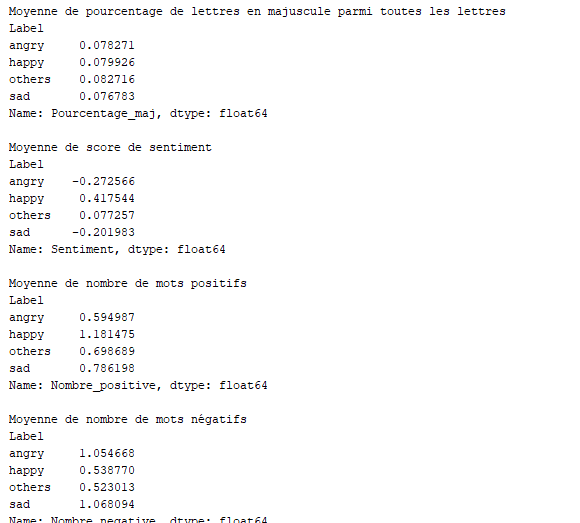
\includegraphics[width=\linewidth,height=15cm,keepaspectratio]{images/analyse_maj_sentiment}

Le score de sentiment utilisé est calculé avec \emph{Senti Word Net} en sommant les valeurs de sentiment attribuées à chaque mot de l'échange de textos. Le nombre de mots positifs/négatifs est calculé en comptant le nombre de mots avec des valeurs de sentiment supérieur/inférieur à 0.

On constate que le pourcentage de lettre majuscule dans les textos est similaire pour toutes les classes, on aurait pu penser qu'il aurait été plus haut pour les textos fâchés. 

Les 3 variables associées aux sentiments semblent beaucoup parler. En effet, les catégories triste et fâché ont des connotations beaucoup plus négatives, alors que la classe joyeuse a beaucoup plus de mots positifs. Cela n'est pas très surprenant.

\subsection{Choix des variables à ajouter} \label{subsec:variables}
On peut maintenant décider quelles variables supplémentaires nous ajouterons dans notre modèle. 
La sélection des variables s'est de façon assez subjective en analysant les comptes des attributs présentés dans la section \nameref{sec:analyse_prelim} et en ajoutant les attributs qui semblaient avoir le plus grand pouvoir discriminant.
Voici la liste des variables ajoutées:

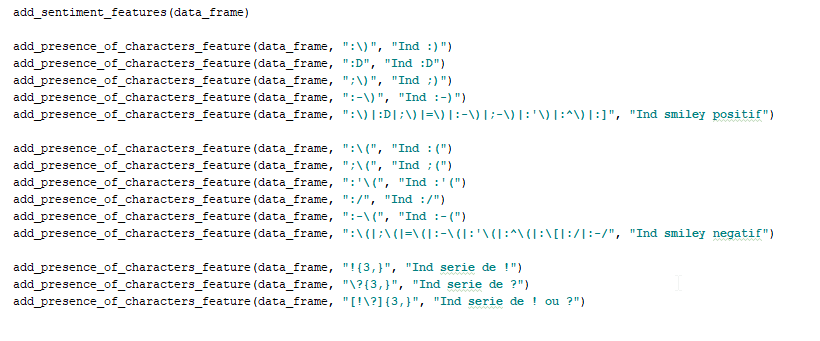
\includegraphics[width=\linewidth,height=14cm]{images/variables_autres}

La fonction \verb|add_sentiment_features| ajoute les 3 variables de sentiments, la fonction \verb|add_presence_of_characters_feature| ajoute un 1 si l'expression régulière donnée en argument est trouvée dans l'échange de textos, 0 sinon. Ainsi, les variables de sentiments, des indicateurs de \emph{smileys} positifs, négatifs et de séries de ponctuations sont ajoutés comme variables.

En conclusion, lorsqu'on roule le code avec \verb|bool_ajouter_autres_features=True|, on ajoute les variables décrites ci-dessus et on transforme tous les \emph{emojis} en texte.

%\newpage

\section{Procédure et méthodologie} \label{sec:methodologie}
Pour parvenir à réaliser la tâche, on utilisera un objet de compte fourni dans la librairie \emph{sklearn} avec d'autres variables décrites dans la section \emph{Analyse préliminaire des données}. Ensuite encore avec \emph{sklearn}, nous utiliserons un modèle de classification pour prédire l'émotion dégagée dans les échanges de textos.

Pour simuler un test sur nos données, le corpus d'entraînement fourni dans \emph{train.txt} sera directement séparé en corpus d'entraînement (80\%) et en corpus de test(20\%)  pour pouvoir évaluer la performance de notre modèle. Ainsi, tous les tests seront réalisés avec 80\% des données. À la fin complètement, le meilleur modèle sera entraîné avec les données d'entraînement et de test.

\subsection{Corpus et objets de compte} \label{subsec:corpus}
Pour créer le corpus, nous avons combiné les 3 échanges de textos en un seul texte séparé par des espaces entre chaque texto. Ainsi, cet échange :
\begin{enumerate}
\item Don't worry  I'm girl
\item hmm how do I know if you are
\item What's ur name?
\end{enumerate}
Devient :\textbf{Don't worry  I'm girl hmm how do I know if you are  What's ur name?} . Ce qui forme le premier texte de notre corpus. Le même processus est appliqué à tous les autres textes.

Pour transformer les mots de notre corpus sous une forme numérique, nous testerons 3 approches différentes : le compte de mots, la présence de mots (0 ou 1) et la valeur TF-IDF (term frequency-inverse document frequency). Pour chacune d'entre elles, nous retirerons les mots outils (\emph{stop words}). 
Les paramètres qui seront modifiés pour ces méthodes de vectorisation des textes sont la longueur des n-grammes et la fréquence minimale d'un n-gramme pour être conservé dans le modèle.

Il est noté qu'on conservera toutes les classes de mots et aucun stemming ne sera appliqué étant donné la nature des textes avec lesquels on travaille:

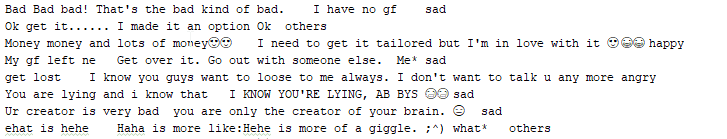
\includegraphics[width=\linewidth,height=5cm]{images/exemples_text}

En effet, on peut voir que certains mots sont inventés, d'autres mal écrits et certains sont des abbréviations. De plus, on voit que certains mots ne sont pas bien séparés par des espaces ce qui fait en sorte que ces algorithmes ne parviendraient pas bien à les séparer. Également, on souhaite limiter le temps de calcul pour l'optimisation de nos hyper-paramètres qui est déjà assez important.

Pour ces raisons, nous avons décidé de ne pas faire de stemming ou de lemmatisation sur nos données textuelles puisque nous jugeons que ces techniques n'apporteraient pas de gains de performance significatifs.

En conclusion, la matrice de données utilisée pour nos modèles de classification sera composée de données d'un des 3 objets de compte décrits dans cette sous-section avec ou sans les attributs supplémentaires décrits dans la section \nameref{sec:analyse_prelim} (si \verb|bool_ajouter_autres_features=True|).

\subsection{Modèles de classification} \label{subsec:modeles}
4 modèles de classification seront testés : SVM, K-PPV, Régression Logistique et MLP. Pour débuter, on peut tester ces modèles avec des paramètres déterminés de façon arbitraire. Pour évaluer le score de performance, on peut utiliser la métrique qui sert à l'évaluation du concours:

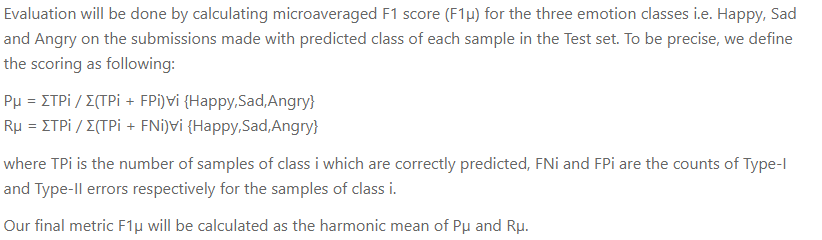
\includegraphics[width=\linewidth,height=10cm,keepaspectratio]{images/metric_concour}

Cette valeur basée sur le nombre de vrais positifs, de faux négatifs et de faux positifs de chaque classe sera calculée 3 fois avec une validation 3-plis sur nos données d'entraînement.
\begin{equation}
F1_{u} =\frac{2}{\frac{1}{P_{u}}+\frac{1}{R_{u}}}
\end{equation}

On peut tester les modèles suivants avec nos objets de compte 1 gram avec occurrence minimale de 40:
\begin{description}
\item \textbf{SVM}(Support Vector Machine): avec paramètres par défaut.
\item \textbf{KPPV} (K plus proche voisins): avec 5 voisins.
\item \textbf{Régression Logistique}: avec paramètres par défaut. (Un contre tous pour le cas multivarié)
\item \textbf{MLP} (Multi Layer Perceptron): avec 2 couches cachées de 100 neurones chaque.
\end{description}

Les résultats ainsi obtenus sont présentés dans la figure \ref{table:modeles_classification}.

% Please add the following required packages to your document preamble:
% \usepackage{multirow}
% \usepackage{longtable}
% Note: It may be necessary to compile the document several times to get a multi-page table to line up properly
\begin{longtable}[c]{cccc}
	\caption{Scores F1 de nos modèles de classification}
	\label{table:modeles_classification}\\
	\hline
	&                       & \multicolumn{2}{c}{\textbf{Score F1}}                             \\ 
	\endhead
	%
	\cline{2-4}
	\endfoot
	%
	\endlastfoot
	%
	\textbf{Vectorisation des mots}     & \textbf{Modèle}       & \textbf{Sans ajout de features} & \textbf{Avec ajout de features} \\ \hline
	\multirow{4}{*}{Word Count}         & SVM & 0,3457 & 0,3710 \\ 
	& k-PPV                 & 0,3836 & 0,4456 \\
	& Régression logistique & 0,5958 & 0,6610 \\
	& MLP                   & 0,5440 & 0,6114 \\ \hline
	\multirow{4}{*}{Word Count binaire} & SVM & 0,3223 & 0,3284 \\ 
	& k-PPV                 & 0,3727 & 0,4040 \\
	& Régression logistique & 0,6046 & 0,6797 \\
	& MLP                   & 0,5428 & 0,6141 \\ \hline
	\multirow{4}{*}{TF-IDF}             & SVM & 0,0229 & 0,0339 \\
	& k-PPV                 & 0,4440 & 0,4482 \\
	& Régression logistique & 0,5833 & 0,6552 \\
	& MLP                   & 0,5443 & 0,6115 \\ \hline
\end{longtable}

On remarque que peu importe le modèle, l'ajout d'autres features que celles de comptes augmente le score du modèle. Les 3 objets de compte semblent avoir des scores similaire d'un modèle à l'autre, on ne peut pas facilement en distinguer un qui sort du lot. Pour ce qui est des modèles de classification, le modèle de régression logistique semble mieux performer que les autres. Cela est probablement dû au fait que les autres modèles ont plus de paramètres à optimiser pour arriver à de bons résultats contrairement à la régression logistique qui en a peu (voir pas).

\subsection{Optimisation de paramètres} \label{subsec:optimisation}
Pour optimiser tous nos paramètres, autant pour les objets de compte que pour les modèles de classification, on calcule le score défini à la section précédente pour plusieurs combinaisons de paramètres possibles. Voici les paramètres choisis pour ces tests:

\begin{description}
\item \textbf{SVM}(Support Vector Machine): valeur de C, type de noyau (kernel)
\item \textbf{KPPV} (K plus proche voisins): nombre de voisins k, type de poids
\item \textbf{Régression Logistique}: type de pénalité appliquée
\item \textbf{MLP} (Multi Layer Perceptron): nombre de neurones pour chaque couche cachée.
\end{description}
Voici les listes des valeurs choisies pour notre recherche en grille:

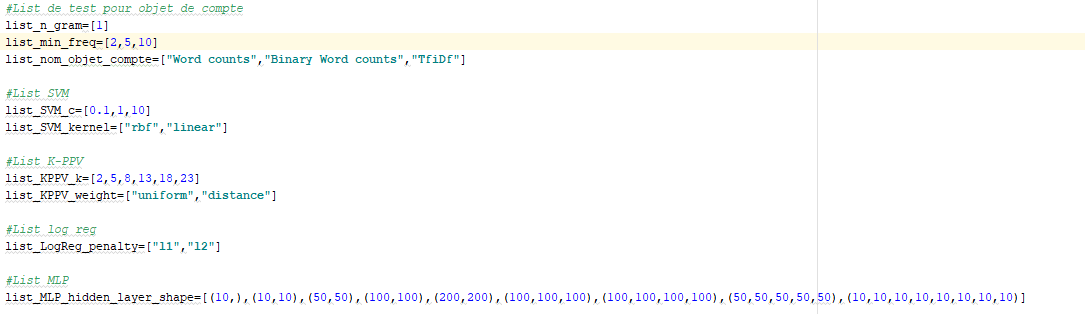
\includegraphics[width=\linewidth,height=8cm]{images/list_param}

Cela fait donc $(1*3*3) *(3*2 + 6*2 + 2 + 9)=261$ combinaisons de paramètres à tester. La combinaison ayant le meilleur score est sauvegardée dans le fichier \emph{Dictionnaire\_parametre\_meilleur\_model} sous la forme d'un dictionnaire contenant ses paramètres. 
Le dictionnaire prend la forme suivante: \{nom du classificateur, score, dictionnaire de paramètres du classificateur, nom du modèle de compte, dictionnaire de paramètres du modèle de compte\}.

\subsection{Test du modèle} \label{subsec:test}
Pour tester notre modèle, on charge le dictionnaire avec nos meilleurs paramètres contenus sur \emph{Dictionnaire\_parametre\_meilleur\_model}. On entraîne le modèle sur l'ensemble de notre 80\% de données séparées au tout début et on prédit le 20\% jamais touché lors de notre optimisation ou entraînement. Le meilleur modèle et les résultats sont présentés à la prochaine section.

%\newpage

\section{Résultats et conclusions} \label{sec:resultats}
\subsection{Simulation de prédictions} \label{subsec:simulation}
Après optimisation, on obtient que le modèle ayant le mieux performer en validation est un celui avec un objet de compte binaire (0 ou 1) qui utilise des 1 gramme et qui conserve une fréquence minimale de 2 mots. Le modèle de classification utilisé est une régression logistique avec une pénalité de choix de paramètres \emph{L1}:

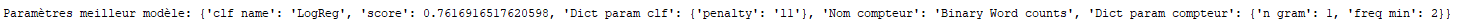
\includegraphics[width=\linewidth,height=1cm,keepaspectratio]{images/dict_meilleur_model}

On peut évaluer notre modèle en calculant le score qu'on obtiendrait sur 80\% de notre corpus d'entraînement qui sert d'entraînement, et 20 \% qui sert de test. Avec notre meilleur modèle, on obtient les résultats suivants:

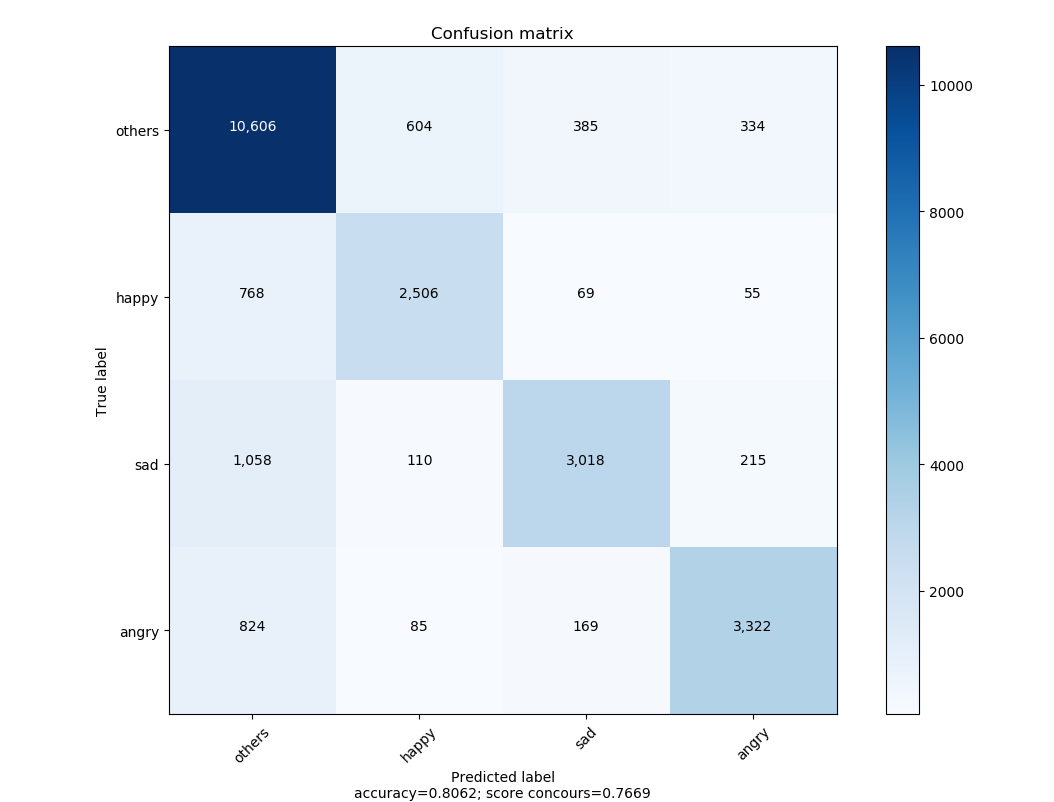
\includegraphics[width=\linewidth,keepaspectratio]{images/confusion_matrix_avec_features}

On peut voir que le score utilisé par le concours de 0.7669 est quand même assez haut. On remarque que la plupart des erreurs faites sont majoritairement de prédire happy, sad et angry comme étant others. De plus, la confusion entre sad et angy est un peu plus élevée qu'entre les autres paires d'émotions puisque qu'on peut supposer que les deux sont à caractère négatif.

On peut également observer la matrice de confusion lorsque l'on n'ajoute pas les variables d'emoji et de binettes:

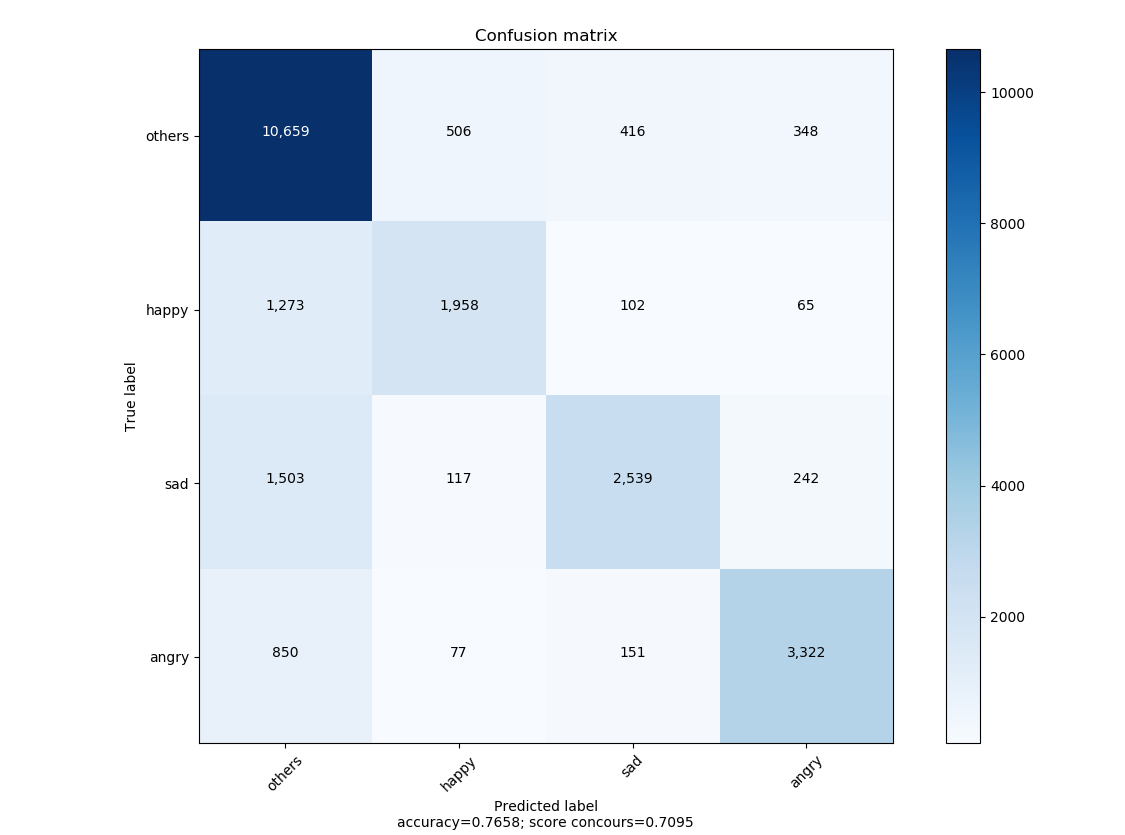
\includegraphics[width=\linewidth,keepaspectratio]{images/confusion_matrix_sans_features}
On voit tout de suite que le score est beaucoup moins bon (0.7095 au lieu de 0.7669). On peut voir que beaucoup plus de classe happy et sad ont été prédites comme étant others (768 à 1273 et 1058 à 1503). Pour ce qui est de angry, les nombres changent très peu, on peut  supposer qu'il y a très peu d'emojis et de binettes dans notre corpus de test pour la classe angry.

Encore une fois, on peut supposer que notre modèle avec les variables ajoutées est meilleur que celui sans, à cause du meilleur score. On peut également comparer notre score aux meilleurs scores soumis à la compétition:

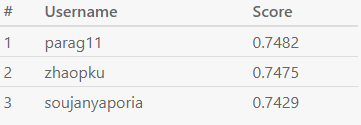
\includegraphics[width=\linewidth,height=4cm,keepaspectratio]{images/meilleurs_scores}

On peut conclure qu'un score de 0.7669 en simulation de test est donc très bon. Il est toutefois difficile de bien comparer puisque la répartition des classes n'est pas la même dans le corpus à prédire. Le fichier de test avait environ 16.6\% de happy, sad, angry et 50\% de others, alors que le fichier à prédire a des proportions de 4\% et 88\%. 

On peut quand même être réellement satisfait du résultat puisque cela ne devrait pas trop affecter nos prédictions.

\subsection{Prédictions sur le jeu de test} \label{subsec:predictions}
On peut observer nos prédictions sur le jeu de test en entraînant notre modèle sur le jeu d'entraînement au complet. Voici les 30 premières prédictions:

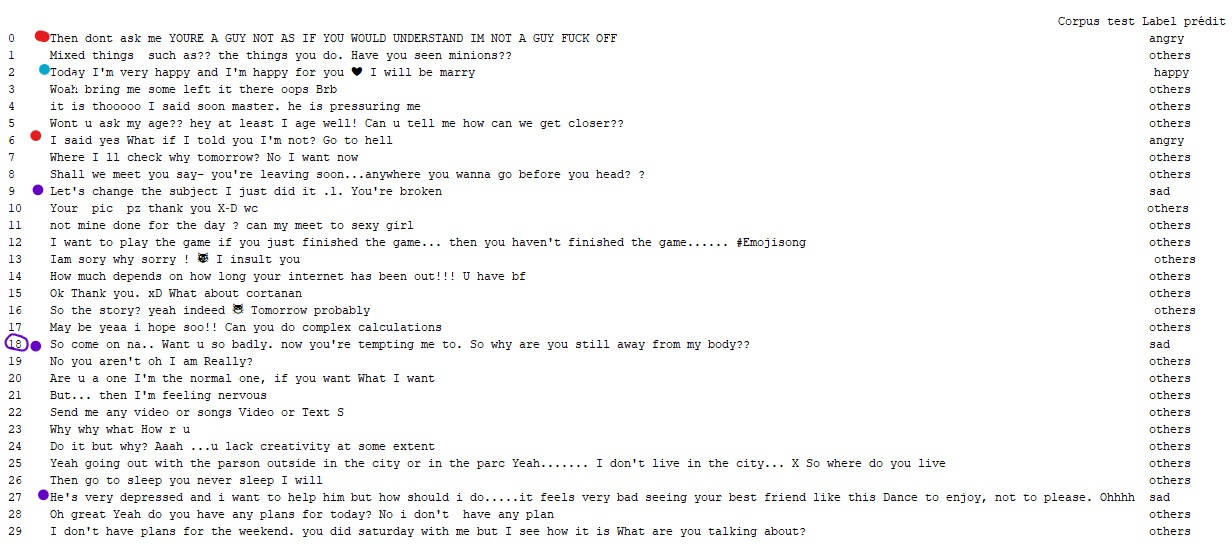
\includegraphics[width=\linewidth,keepaspectratio]{images/couleur_predictions}

Il est difficile d'analyser facilement nos prédictions puisqu'on n'a pas les classes à notre disposition. 

On peut toutefois voir qu'à tous ceux pour lesquels on prédit soit happy/angry/sad, les prédictions semblent bonnes sauf pour le numéro 18 qui n'a clairement pas l'air triste. On peut supposer que cet échange cocasse est mal classé à cause de "Want u so badly". En effet, le mot \emph{"badly"} a une forte connotation négative, ce qui induit notre modèle à classer ce texte en tant que triste. 

En regardant rapidement, on peut voir que ceux classés comme \emph{others} ont l'air particulièrement neutre, sauf peut-être le 13, mais cela est assez subjectif.

Ce petit échantillon nous laisse avec une très bonne impression de notre modèle.

%\newpage

\section{Améliorations et retrospective sur le projet réalisé} \label{sec:ameliorations}
\subsection{Améliorations possibles} \label{subsec:ameliorations}
Plusieurs améliorations ou changements pourraient être effectués pour réaliser ce projet, en voici quelques uns:

\begin{enumerate}
\item Lors de la création du corpus, on considère l'échange de 3 textos comme un gros bloc de texte. Il pourrait être intéressant de tenter de trouver une relation entre les échanges qui pourrait aider à faire une meilleure classification.

\item Un gros problème du projet réalisé est le problème de \emph{"runtime"} du code. En effet, l'ajout de variables de sentiment dans les attributs augmente terriblement le temps d'exécution du code. Il faudrait revoir en entier les fonctions qui y sont associées.

\item Un travail plus exhaustif et robuste pourrait être fait sur les binettes ajoutées comme variables. On pourrait faire un modèle qui analyse toutes les chaînes de caractères spéciaux et qui détermine le degré de signification de chacune pour toutes nos classes.

\item Dans l'optimisation de paramètres, on pourrait tester un nombre de n gramme supérieur à 1.
\end{enumerate}

\subsection{Apprentissage} \label{subsec:apprentissage}
Ce fut un projet très intéressant qui permet d'appliquer plusieurs connaissances en traitement de langue naturelle. Il permet d'appliquer les notions de classification de textes, d'analyse de sentiment et les expressions régulières.
Également, contrairement aux autres projets réalisés au cours de la session, ce projet laissait libre cours à notre imagination et nous avions la liberté d'expérimenter avec plusieurs approches pour résoudre un même problème.

L'utilisation d'emojis et de binettes pour classer les échanges de textos était également très intéressante puisqu'elle n'a pas été vue en classe, mais apporte tout de même une quantité non-négligeable d'information à notre modèle.

Le projet fut également très formateur pour les auteurs du code Python qui contrairement à leur habitude, ont tenté de faire un code plus lisible et réutilisable pour d'autres applications. 


%\newpage

\section{Annexe} \label{sec:annexe}
\subsection{Liste de scores d'optimisation} \label{subsec:scores}
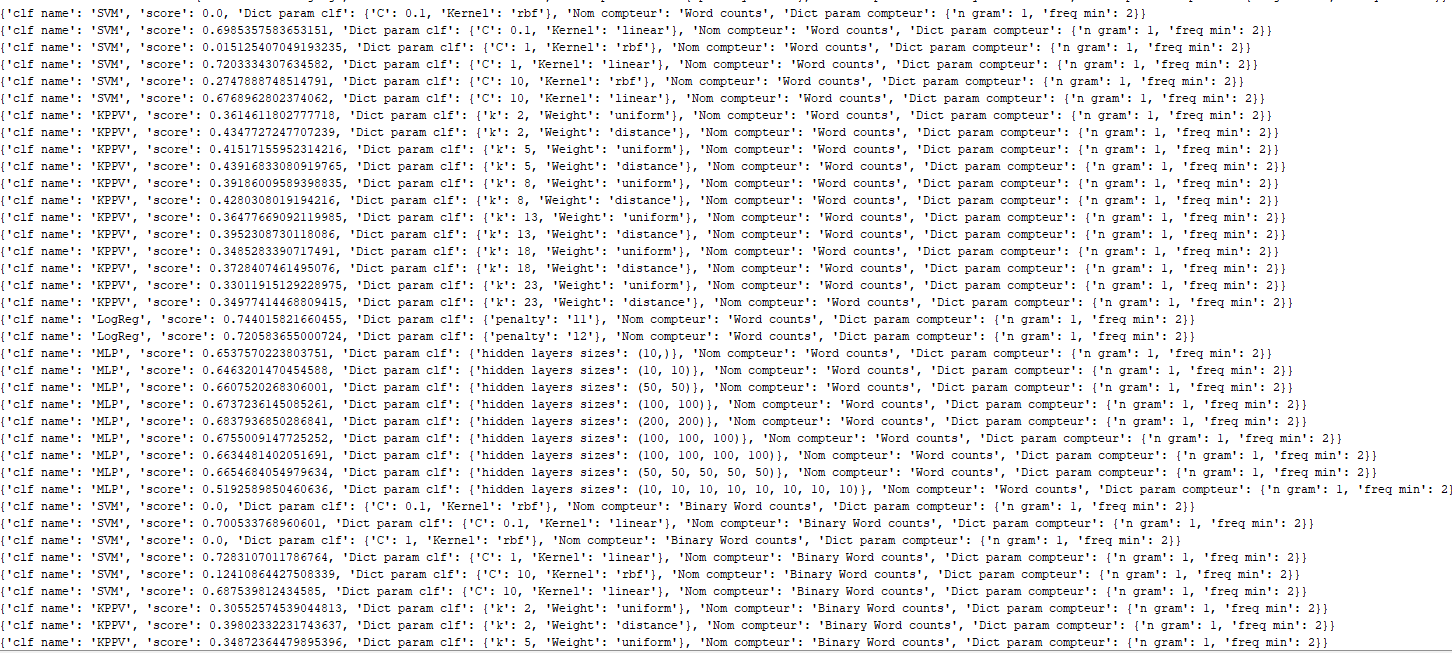
\includegraphics[width=\linewidth,height=12cm,keepaspectratio]{images/page_1}

Le reste des pages peuvent être "\emph{print}" avec le code, avec \verb|bool_print_tous_models_optimisation|

\end{document}

